\documentclass{article}
\usepackage{tikz}
\usetikzlibrary{positioning}
\begin{document}
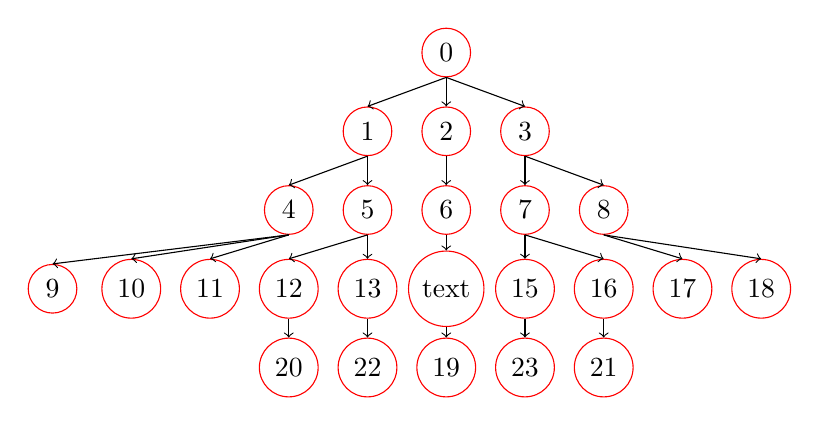
\begin{tikzpicture}
\node[circle, draw=red] (node_0_0) [] at (0,0) {0};
\node[circle, draw=red] (node_-1_-1) [] at (-1,-1) {1};
\draw[->] (node_0_0.south) --  (node_-1_-1.north);
\node[circle, draw=red] (node_0_-1) [] at (0,-1) {2};
\draw[->] (node_0_0.south) --  (node_0_-1.north);
\node[circle, draw=red] (node_1_-1) [] at (1,-1) {3};
\draw[->] (node_0_0.south) --  (node_1_-1.north);
\node[circle, draw=red] (node_-2_-2) [] at (-2,-2) {4};
\draw[->] (node_-1_-1.south) --  (node_-2_-2.north);
\node[circle, draw=red] (node_-1_-2) [] at (-1,-2) {5};
\draw[->] (node_-1_-1.south) --  (node_-1_-2.north);
\node[circle, draw=red] (node_0_-2) [] at (0,-2) {6};
\draw[->] (node_0_-1.south) --  (node_0_-2.north);
\node[circle, draw=red] (node_1_-2) [] at (1,-2) {7};
\draw[->] (node_1_-1.south) --  (node_1_-2.north);
\node[circle, draw=red] (node_2_-2) [] at (2,-2) {8};
\draw[->] (node_1_-1.south) --  (node_2_-2.north);
\node[circle, draw=red] (node_-5_-3) [] at (-5,-3) {9};
\draw[->] (node_-2_-2.south) --  (node_-5_-3.north);
\node[circle, draw=red] (node_-4_-3) [] at (-4,-3) {10};
\draw[->] (node_-2_-2.south) --  (node_-4_-3.north);
\node[circle, draw=red] (node_-3_-3) [] at (-3,-3) {11};
\draw[->] (node_-2_-2.south) --  (node_-3_-3.north);
\node[circle, draw=red] (node_-2_-3) [] at (-2,-3) {12};
\draw[->] (node_-1_-2.south) --  (node_-2_-3.north);
\node[circle, draw=red] (node_-1_-3) [] at (-1,-3) {13};
\draw[->] (node_-1_-2.south) --  (node_-1_-3.north);
\node[circle, draw=red] (node_0_-3) [] at (0,-3) {text};
\draw[->] (node_0_-2.south) --  (node_0_-3.north);
\node[circle, draw=red] (node_1_-3) [] at (1,-3) {15};
\draw[->] (node_1_-2.south) --  (node_1_-3.north);
\node[circle, draw=red] (node_2_-3) [] at (2,-3) {16};
\draw[->] (node_1_-2.south) --  (node_2_-3.north);
\node[circle, draw=red] (node_3_-3) [] at (3,-3) {17};
\draw[->] (node_2_-2.south) --  (node_3_-3.north);
\node[circle, draw=red] (node_4_-3) [] at (4,-3) {18};
\draw[->] (node_2_-2.south) --  (node_4_-3.north);
\node[circle, draw=red] (node_-2_-4) [] at (-2,-4) {20};
\draw[->] (node_-2_-3.south) --  (node_-2_-4.north);
\node[circle, draw=red] (node_-1_-4) [] at (-1,-4) {22};
\draw[->] (node_-1_-3.south) --  (node_-1_-4.north);
\node[circle, draw=red] (node_0_-4) [] at (0,-4) {19};
\draw[->] (node_0_-3.south) --  (node_0_-4.north);
\node[circle, draw=red] (node_1_-4) [] at (1,-4) {23};
\draw[->] (node_1_-3.south) --  (node_1_-4.north);
\node[circle, draw=red] (node_2_-4) [] at (2,-4) {21};
\draw[->] (node_2_-3.south) --  (node_2_-4.north);
\end{tikzpicture}
\end{document}
